\documentclass[a4paper,12pt]{article}
\usepackage[OT4,plmath]{polski}
\usepackage[utf8x]{inputenc}
\usepackage{url}

\usepackage{a4wide}
\usepackage{hyperref}
\usepackage{caption}
\usepackage{graphicx}

\graphicspath{ {imgs/} }

\title{{\textbf{Skalowanie baz danych na przykładzie MySQL}}}
\author{Rafał Łasocha}
\date{Wrocław, dnia \today\ r.}

\begin{document}

\maketitle

\section{Skalowanie systemów informatycznych}

Dla wielu aplikacji wystarczający jest tylko jeden serwer bazodanowy. Niektóre z nich jednak zbierają tyle informacji, że prędzej czy później dochodzą do momentu, w którym dane nie mieszczą się na jednym serwerze i jest konieczność zmian w infrastrukturze, żeby te dane pomieścić.

\subsection{Co to znaczy, że system jest skalowalny?}

Twórcy usług bazodanowych (lub innych usług, z których korzystają programiści), często posługują się terminem „skalowalność” w odniesieniu do ich produktów. Poza tym, że używają tego słowa sprzedawcy, żeby reklamować swój produkt, można ten termin w miarę konkretnie zdefiniować. 

Najpierw jednak zdefiniujmy pojęcie „wydolności” systemu. Oczywiście, dokładna definicja jak bardzo wydolny jest system baz danych, w dużej mierze zależy od jego wykorzystania.  Różne aplikacje mają różny stosunek zapisów do odczytów, różne wielkości tabel (w niektórych systemach wszystkie tabele są mniej więcej jednakowo duże, w innych jest tylko kilka tabel które składają się na większość systemu i to wydajność odczytów/zapisów tych kilku tabel próbujemy zoptymalizować) itd. Intuicyjnie możemy myśleć o wydolności w ten sposób: jak dużą możemy osiągnąć przepustowość (w liczbie zapytaniach na sekundę na przykład) utrzymując rozsądny czas odpowiedzi.

Dla przykładu, typowe testy wydajnościowy w stylu „wyślemy 1000000 zapytań SQL i policzymy czas, w którym serwer się wyrobi z obsłużeniem wszystkich” to nie jest do końca to, co nas interesuje, bo w takim przypadku serwer będzie przetwarzał zapytania pod maksymalnym obciążeniem. Nas interesuje test „będziemy wysyłać 1000 zapytań na minutę, i dostaniemy odpowiedź poniżej 3ms w 90\% przypadków”. Co trzeba podkreślić, wydolność bardzo zależy od naszego systemu, bo te „1000 zapytań na minutę”, to nie są dowolne zapytania, tylko takie, które występują w naszej aplikacji. Stąd, na wydolność naszej aplikacji ma wpływ liczba użytkowników, wielkość przetrzymywanych danych na serwerze, wielkość przetrzymywanych danych w przeliczeniu na jednego użytkownika („prawo papieża”: zawsze może być w naszej aplikacji kilka użytkowników, na których przypada nieproporcjonalnie dużo danych – i to też musimy wziąć pod uwagę, bo papież również chciałby korzystać swobodnie z naszej aplikacji).

Jeśli już rozumiemy pojęcie wydolności, które możemy jakoś określić dla konkretnej skonfigurowanej maszyny („wydolność naszego systemu to 1000 zapytań na minutę”), to oczywistym dla nas jest, że wiele aplikacji w swoim cyklu rozwoju ma taki moment, że potrzebuje zwiększyć tę wydolność.

I tutaj możemy przejść do definicji skalowalności. Skalowalność mówi nam, do jakiego stopnia zwiększa nam się wydolność systemu, gdy dodajemy kolejne serwery. Pierwszą naszą myślą może być, że gdy mamy 1 serwer i dodamy drugi, to wydolność zwiększy się o 100\% (skalowalność liniowa – \ref{fig:scaling-linear}). Oczywiście zdrowy rozsądek podpowiada nam, że każdy taki serwer ma jakiś stały narzut na swoje działanie, więc prawdopodobnie skalowalność jest krzywą trochę poniżej liniowej (\ref{fig:scaling-almost-linear}). Skalowalność wielu systemów wygląda właśnie w ten sposób i wzięcie pod uwagę stałego „kosztu” na każdy serwer nazywamy prawem skalowalności Amdahla.

\begin{figure}[ht]
\centering
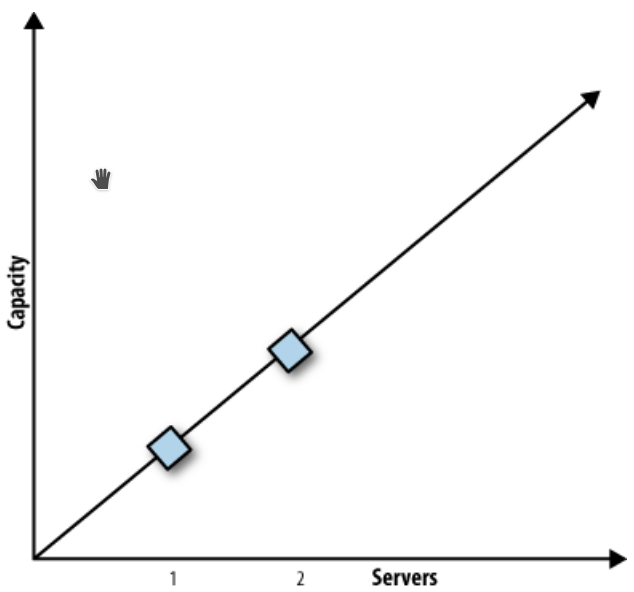
\includegraphics[width=0.5\textwidth]{scaling-linear.png}
\caption{Skalowalność liniowa}
\label{fig:scaling-linear}
\end{figure}

\begin{figure}[ht]
\centering
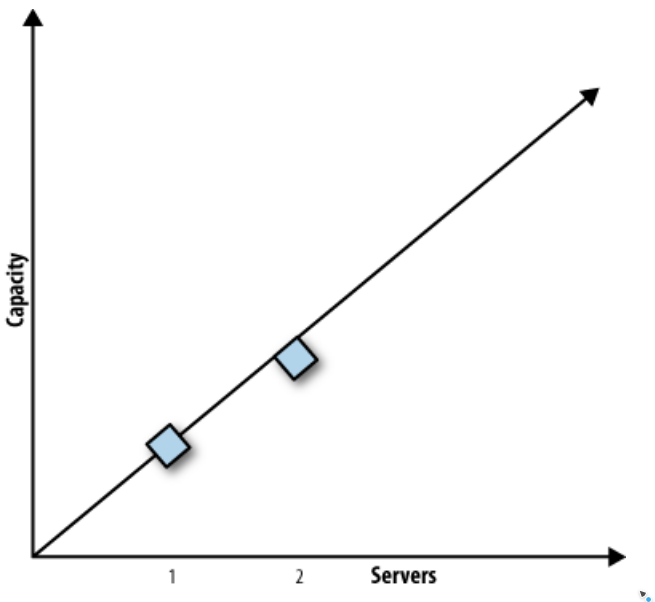
\includegraphics[width=0.5\textwidth]{scaling-almost-linear.png}
\caption{Skalowalność ze stałym narzutem na serwer}
\label{fig:scaling-almost-linear}
\end{figure}

Jeszcze zdrowszy rozsądek podpowie nam, że taki system na pewno ma jakieś granice, do którego możemy dokładać dodatkowe serwery i ciągle mieć z tego zysk. Dlatego też jest uniwersalne prawo skalowalności, które bierze również pod uwagę fakt, że serwery w danym systemie mogą potrzebować wymieniać ze sobą informacje (na zasadzie „każdy z każdym”). To powoduje, że mamy narzut $N^2$ do wydolności na każdym serwerze, więc jest taki moment, gdzie dołożenie kolejnego serwera pogorszy wydolność całego systemu (\ref{fig:scaling-all})!

\begin{figure}[ht]
\centering
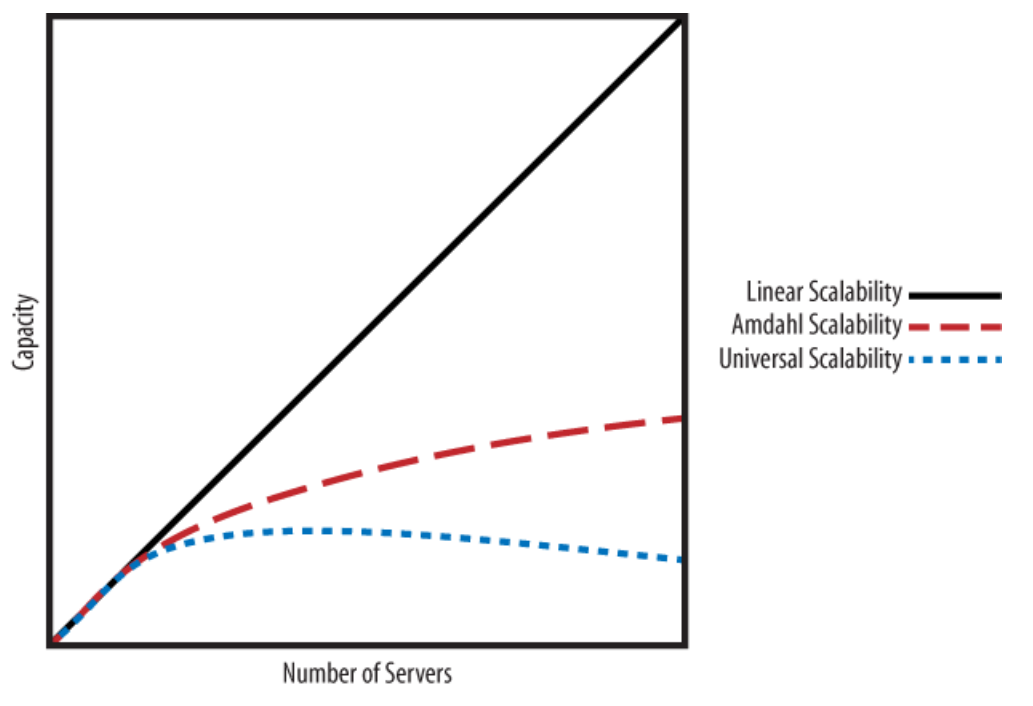
\includegraphics[width=0.7\textwidth]{scaling-all.png}
\caption{Wszystkie popularne rodzaje skalowalności}
\label{fig:scaling-all}
\end{figure}


Większość systemów stosuje się właśnie do uniwersalnego prawa skalowalności. Oczywiście jak każdy model, jest to tylko przybliżenie – niektóre systemy mogą nie potrzebować akurat $N^2$ narzutu na komunikację, tylko dowolną inną funkcję, a może się zdarzyć też, że skalowalność będzie większa niż liniowa (rozpatrzmy przypadek gdzie mamy jeden serwer, który ma obciążony zarówno pamięć jak i dysk twardy i system operacyjny ciągle „swapuje”, po czym dokładamy drugi serwer, dzięki któremu wszystkie dane mieszczą się w pamięci RAM).

\subsection{Skalowanie MySQL}

Rozważymy dwa sposoby na skalowanie systemu bazodanowego – skalowanie pionowe i skalowanie poziome. Skalowanie pionowe polega na tym, że ciągle mamy tylko jeden serwer, ale zwiększamy jego parametry (pamięć RAM, liczba CPU), żeby był bardziej wydolny. W skalowaniu poziomym, zwiększamy liczbę maszyn.

\section{Skalowanie pionowe}

Skalowanie pionowe jest świetnym rozwiązaniem aby kupić sobie trochę czasu. Jeśli jeszcze nie wiemy czy nasza aplikacja odniesie sukces, skalowanie pionowe jest lepszym wyborem, bo kosztuje znacznie mniej – zmiana maszyny na lepszą jest znacznie prostszą operacją niż skonfigurowanie całej infrastruktury, przygotowanie aplikacji do korzystania z wielu serwerów, przygotowanie procedur tworzenia/przywracania kopii zapasowych itd. A jako że z reguły najdroższą rzeczą w firmie są wynagrodzenia pracowników IT, to skalowanie pionowe jest bardziej opłacalne.

Główną wadą skalowania pionowego jest fakt, że nie można go robić w nieskończoność. Parametry serwerów mają swoje rozsądne granice, i im lepsze serwery kupujemy, tym droższe robią się zasoby, więc w pewnym momencie zaczyna się opłacać przejście na skalowanie poziome. Poza tym, musimy pilnować aby aktualizować wersję MySQLa – nie możemy oczekiwać, żeby kod napisany i testowany np. 10 lat temu działał wydajnie na systemie z 256GB RAMu – nikt wtedy nie miał możliwości przetestować bazy danych na takim sprzęcie.

\section{Skalowanie poziome}

Skalowanie poziome możemy podzielić na trzy rodzaje: replikację, dzielenie funkcjonalne i sharding. Replikacja jest najprostszą formą i pozwala przenieść część odczytów na inne serwery, ale nie pomoże nam, jeśli naszym wąskim gardłem są zapisy. Zarówno dzielenie funkcjonalne jak i sharding rozwiązuje problem wydolności zapisów.

\section{Dzielenie funkcjonalne}

Dzielenie funkcjonalne jest prostym pomysłem, niewiele mającego wspólnego z konkretną bazą danych i jej możliwościami (w przeciwieństwie do np. replikacji, która musi być wspierana przez bazę danych, żeby ją efektywnie zrobić). Jeśli nasza aplikacja jest niewydolna żeby jeden serwer ją utrzymał, to jest spora szansa, że jest bardzo duża - duża, w sensie liczby różnych funkcjonalności, a nie liczbie użytkowników. Możemy ją więc podzielić, ze względu na 	zestawy funkcjonalności, jeśli te części kodu korzystają z raczej rozdzielnych zestawów tabel. Mówię „raczej”, bo prawdopodobnie każda korzysta z tabeli użytkowników.

Wyobraźmy sobie jakiś serwis informacyjny. Możemy bazę danych pociąć na kilka oddzielnych dużych funkcjonalności: witryna z bieżącymi wiadomościami, forum dla czytelników, helpdesk i właśnie baza użytkowników. Udało nam się więc podzielić, niewielkim kosztem serwis na kilka baz danych i prawdopodobnie osiągnąć  skalowalność bliską liniowej (bazy danych są całkowicie rozłączne i nie komunikują się ze sobą). Jak widać dzielenie funkcjonalne jest względnie proste (w porównaniu do shardingu, który opisany będzie w dalszej części artykułu) i nie niesie ze sobą zbyt wielu zagrożeń (w momentach gdzie rzeczywiście musimy porozmawiać z więcej niż jedną bazą danych, być może musimy się pogodzić z brakiem transakcyjności – ale jeśli dzielenie funkcjonalne jest zrobione poprawnie, to są to rzadkie przypadki).

Koniec końców niestety, w naszej aplikacji najprawdopodobniej jest takich rozdzielnych modułów kilka, albo kilkanaście, więc nie możemy dzielić w ten sposób naszej aplikacji zbyt długo. W szczególności, może okazać się, że tylko jeden z tych już rozdzielonych baz danych potrzebuje bardziej skomplikowanego rozwiązania (shardingu), więc z reguły dzielenie funkcjonalne idzie w parze z shardingiem i sharding tego podziału nie likwiduje.

\section{Sharding}

Jest to aktualnie najpopularniejsza metoda skalowania bazy danych MySQL. Wystarczy wspomnieć, że korzystają z tego rozwiązania takie firmy jak Facebook, Instagram czy Uber. Jak wspomniane zostało wyżej, sharding idzie w parze z dzieleniem funkcjonalnym. Z reguły jest jakaś baza danych, która trzyma dane globalne, które są potrzebne wszystkim (np. właśnie listę użytkowników), często broniona przez klaster szybkiego cache, np. memcached. Aplikacje które korzystają z bazy danych z shardingiem, raczej o tym wiedzą. Potrzebna jest jakaś programistyczna abstrakcja, która decyduje do jakiego serwera bazodanowego wysłać żądania SQL. Można to zrobić tak, żeby aplikacja nie wiedziała z kim rozmawia, ale jest to niewskazane. Równomierna (ilościowo) dystrybucja danych po wszystkich serwerach jest nieefektywna (co pokażemy później), więc chcemy robić to trochę mądrzej.

\subsection{Wybór klucza shardującego}

Jeśli uznamy że potrzebujemy shardingu, jedną z pierwszych decyzji do podjęcia jest wybór klucza shardującego. Klucz ten decyduje, na jakim shardzie wyląduje rekord. W MySQL NDB Cluster, który jest gotowym rozwiązaniem do wdrażania shardowanej bazy danych, rekordy są równomiernie rozprowadzane po serwerach wg haszowanego klucza głównego w danej tabeli. To proste rozwiązanie, ale z nienajlepszą wydajnością.

Wyobraźmy sobie platformę blogową, gdzie użytkownicy mają posty i piszą komentarze pod postami innych autorów. Żeby wyświetlić stronę główną takiego bloga, musimy pobrać wszystkie posty danego użytkownika. Skoro posty są rozłożone równomiernie na wszystkich serwerach, to musimy zrobić (najlepiej równolegle) zapytania do wszystkich serwerów i potem połączyć te dane (dodatkowe utrudnienia: co jeśli zapytanie miało klauzulę \texttt{ORDER BY}, \texttt{LIMIT}, \texttt{HAVING} - to wszystko musi być wtedy obsłużone w abstrakcji programistycznej po stronie klienta). Jest to zrobienia, ale może da się tutaj zrobić coś lepiej. Dlatego najczęściej dobrym kluczem jest identyfikator użytkownika (jeśli pomyślimy np. o witrynie społecznościowej) lub identyfikator klienta (częste w aplikacjach modelu SaaS, gdzie jest zakładane konto dla całej firmy i wiele kont użytkownika podlega pod tą firmę).

Mamy tutaj jeszcze inny problem. Załóżmy że mamy dwa widoki:
\begin{itemize}
 \item wyświetlenie posta ze wszystkimi komentarzami pod spodem
 \item wyświetlenie profilu użytkownika, ze wszystkimi jego komentarzami
\end{itemize}
Jak w takim wypadku rozprowadzać komentarze po serwerach? Możemy to zrobić wg identyfikatora użytkownika lub identyfikatora posta, ale wtedy zawsze jeden z powyższych widoków będzie wymagał zapytań do wszystkich serwerów. Częstym rozwiązaniem tutaj jest denormalizacja i duplikacja danych. Oczywiście, trzymanie zduplikowanych danych to jest pewien koszt, ale może w naszym przypadku wydajność jest ważniejsza. Można też się zastanowić czy na pewno wszystkie dane o komentarzach są potrzebne w obu zastosowaniach - może w przypadku profilu użytkownika wystarczy wyświetlić jedynie nagłówki komentarzy? Mamy wtedy zaletę że trzymamy dane dokładnie zgodne z ich przeznaczeniem.

\subsection{Zapytania do wielu shardów}

Niezależnie od zastosowanych technik, nie uda się nam wybrać klucza który by idealnie podzielił dane tak, że wszystkie zapytania odwoływałyby się tylko do jednego sharda. Na naszej platformie blogowej, możemy chcieć mieć np. listę najpopularniejszych postów, więc siłą rzeczy musielibyśmy wysłać zapytania do wszystkich shardów. Jest kilka technik do radzenia sobie z takimi zapytaniami:
\begin{itemize}
 \item warstwa cache dla ciężkich zapytań
 \item tabele, które przetrzymują wyniki trudniejszych zapytań - dane o najpopularniejszych postach możemy na bieżąco przetwarzać w tle i wrzucać je do tabeli z wynikami. Taką tabelę z wynikami możemy wtedy albo zduplikować na wszystkich shardach, albo wrzucić w oddzielną bazę danych.
\end{itemize}

Nie tylko zapytania są trudne do zrealizowania w shardowanych bazach danych - jeśli mamy shardy, to tracimy też klucze obce (pomiędzy shardami) i transakcyjność (zależnie od rozwiązania, są sposoby aby transakcyjność odzyskać).

Poza odczytem danych, trudniejsze też może być ich usunięcie - jeśli chcemy usunąć użytkownika, to zamiast robić żądania do wszystkich shardów wykonujące usuwanie danych, możemy tylko dodać użytkownika do usunięcia, a samym usuwaniem danych zajmie się jakiś proces działający w tle.

\subsection{Przydzielanie shardów do serwerów}

Niekoniecznie musi być tak, że na jednym serwerze jest tylko jeden shard z danymi - wprost przeciwnie, zaraz wytłumaczę dlaczego lepszym pomysłem jest posiadanie wielu małych shardów na kazdym serwerze i jakie są zalety i wady obu rozwiązań.

Wyobraźmy sobie że mamy na serwerze 100GB danych - możemy je podzielić na 1 shard 100 GBajtowy lub 100 shardów wielkości 1GB. Pierwszą sprawą którą można wziąć pod uwagę, to zmiany struktury tabel. W MySQL, wiele z operacji zmian struktury blokuje całą tabelę (takie jak np. zmiana długości pola VARCHAR, dodawanie niektórych indexów, dodawanie kolumn w wersji niższej niż 5.6 itd.). Lepiej jest więc aby proces zmiany struktury był robiony po kolei i blokował każdy mały shard na kilka minut, niż żeby jeden duży shard został zablokowany na godzinę. Mniejsze shardy są też łatwe do przenoszenia, bo operacja przeniesienia jednego shardu na drugi jest znacznie prostsza niż operacja rozdzielenia sharda na kilka części.

Są tylko dwie wady małych shardów: po pierwsze, prawdopodobnie rośnie liczba zapytań pomiędzy różnymi shardami (z którymi nauczyliśmy się sobie radzić w poprzedniej sekcji). Drugą wadą jest to, że jeśli mamy aktualnie działającą aplikację i przynoszący pieniądze biznes, operacja rozdzielenia bazy na dwie części (i dodanie infrastruktury do tego) może być znacznie prostsza niż rozdzielenie bazy na 1000 części. W pierwszym przypadku możemy sobie pewnie jeszcze pozwolić na robienie czegoś ręcznie (ale dwa razy), w drugim już musimy zautomatyzować wszystkie operacje działające na bazie danych.

\subsection{Implementacja shardów na serwerach}

Przechodząc bardziej do technicznych szczegółów - jak reprezentować shard danych na serwerze? Jest kilka najpopularniejszych sposobów:

\begin{itemize}
 \item każdy shard jest osobną bazą danych o takiej samej nazwie jak oryginalna
 \item każdy shard jest osobną bazą danych o nazwie z sufiksem numerycznym oznaczającym numer sharda (np. do tabeli z komentarzami odwoływalibyśmy się przez\\ \texttt{bookclub\_23.comments} itd.)
 \item na jednym serwerze jest tylko jedna baza danych, a tabele mają sufiks numeryczny oznaczający numer sharda (np. \texttt{bookclub.comments\_23})
 \item sufiks z nr sharda jest zarówno w nazwie bazy danych, jak i nazwie tabeli \\(\texttt{bookclub\_23.comments\_23})
 \item połączenie dowolnego z powyższych, można też wziąć pod uwagę uruchomienie kilku różnych instancji MySQL na danym serwerze obsługującą pewną liczbę shardów, itd.
\end{itemize}

Wszystkie podane sposoby są łatwe do wprowadzenia w nowej aplikacji, więc tam doradzane jest użycie sufiksu zarówno w tabeli, jak i bazie danych, żeby uniknąć ewentualnych pomyłek i błędów. Jednak jest to też sposób najbardziej inwazyjny dla kodu produkcyjnego. Dodanie numeru sharda tylko do bazy danych jest średnio inwazyjne w kodzie aplikacji - pewnie musimy ten numer gdzieś przekazać przy rozpoczęciu żądania do serwera, ale kod wykonujący zapytania SQL może zostać taki, jaki był przed dodaniem shardingu do aplikacji. Jeśli sufiks jest też w nazwie tabel, to zmian może być znacznie więcej, prawdopodobnie każde zapytanie SQL w systemie będzie musiało być lekko zmodyfikowane.

Podczas rozrzucania shardów po serwerach, warto też wziąć pod uwagę lokalizację użytkownika - jeśli nasza firma jest globalna, użytkowników z Europy można wrzucić do innego DC (zlokalizowanego w Europie), niż użytkowników z Azji.

\subsection{Metody przydzielania rekordów do shardów}

Musimy jakoś rozdzielić wszystkie rekord, pomiędzy różne shardy. Możemy sobie wyobrazić, że mamy znaleźć funkcję która bierze klucz shardujący i przydziela numer sharda.

\subsection{Przydział statyczny}

Pierwszym co przychodzi na myśl, jest jakaś funkcja haszująca i operacja modulo. Przykładowo, jeśli klucz sharda to 111 i mamy 100 shardów, to możemy (pomijając funkcję haszującą) przydzielić temu kluczowi shard 11 ($111 \bmod 100 = 11$). Zaletami tego rozwiązania jest prostota i niski narzut na wydajność i na kod aplikacji. Przydział statyczny ma istotne wady:

\begin{itemize}
 \item jeśli shardów mamy tylko kilka, to ciężko je zbalansować (może się okazać że większość aktywnych użytkowników wyląduje na jednym shardzie)
 \item ciężko zmieniać liczbę shardów, wymagałoby to operacji przenosin wszystkich rekordów na shardy o nowym identyfikatorze, co nie jest prostą sprawą (infrastrukturalnie)
\end{itemize}

Dlatego też, pomimo że wiele firm najpierw zaczyna z przydziałem statycznym (bo jest prosty do zrobienia), to prędzej czy później przechodzi na przydział dynamiczny.

\subsection{Przydział dynamiczny}

Przydział dynamiczny polega na trzymaniu całego mapowania z identyfikatora shardowania do numeru shardu w oddzielnym kontenerze z danymi (np. warstwa memcached, redisa, albo po prostu oddzielna baza danych). Wystarczy pamiętać aby przy dodawaniu nowego użytkownika, dodać też rekord do tego mapowania. Jak widać, dodawanie nowych shardów jest całkowicie trywialne (nie wymaga właściwie żadnej ingerencji w mapowanie), a przenoszenie użytkowników jest znacznie ułatwione. Korzystając z przydziału dynamicznego możemy też sobie pozwolić na posiadanie shardów o różnej wielkości (jeśli akurat jesteśmy w trakcie aktualizacji serwerów do takich o większej mocy). Możemy też optymalizować dane rozmieszczając je dowolnie pomiędzy shardy - być może dzięki temu jesteśmy w stanie zastąpić zapytania które wcześniej musiały być wysłane do wszystkich shardów, do takiego które musi zostać wysłane tylko do kilku (lub jednego - wyobraźmy sobie stronę która wyświetla ranking blogerów z danego kraju - można umieścić blogerów z jednego kraju obok siebie na shardach).

\subsection{Przydział sprecyzowany}

Trzecim podejściem, trochę innych niż dwa poprzednie, jest przydział sprecyzowany. Zamiast robić mapowanie z klucza shardującego do numeru sharda, możemy sprawić żeby numer sharda zawierał się w kluczu shardującym (co trochę przypomina przydział statyczny). W tym celu, zakładając że kluczem shardującym jest identyfikator użytkownika, założyć że np. pierwsze 6 bitów identyfikatora użytkownika to właśnie numer sharda. Otrzymanie numeru sharda lub tej ``rzeczywistej'' części numeru użytkownika to wtedy kwestia prostych operacji bitowych. Istotną zaletą tego rozwiązania jest to, że nie potrzebujemy żadnego dodatkowego zapytania aby otrzymać numer sharda. Jest to jakieś rozwiązanie pośrednie pomiędzy przydziałem stałym i dynamicznym, bo możemy częściowo sterować gdzie są nasze rekordy (podejmujemy decyzję o tym przy dodawaniu rekordu) oraz łatwo jest zwiększyć liczbę shardów, które używamy. Wadą jest, podobnie jak w przydziale statycznym, trudność w przesuwaniu danych pomiędzy shardami - jeśli dany rekord wyląduje w jakimś shardzie, to ciężko go będzie stamtąd ruszyć.

\section{Podsumowanie}

Omówiliśmy w tym artykule kilka technik skalowania bazy danych na przykładzie MySQL, zalety i wady skalowania pionowego i poziomego i różnego rodzaju decyzji które trzeba podjąć przy skalowaniu poziomym.

Ciężko mi się odnieść do całego tematu skalowania z doświadczenia zawodowego - największej aplikacji przy której aktualnie pracuję, wystarcza (już niedługo, ale jeszcze) 16GB pamięci RAM i około 50GB dysku twardego. Sporo jeszcze czasu minie, zanim dojdziemy do momentu gdzie skalowanie pionowe i dzielenie funkcjonalne to będzie za mało.

\section{Źródło}

Seminarium i referat na podstawie własnych doświadczeń z programowaniem aplikacji korzystających z baz danych i 11 rozdziału z książki Baron Schwartz, Peter Zaitsev, Vadim Tkachenko, ``High Performance MySQL'', 3rd Edition, O'Reilly 2012

\end{document}
